\subsection*{Zadania: Środki ciężkości}

Wyznacz położenie środków ciężkości płaskich arkuszy blach. W przypadku blach niejednorodnych uwzględnij różnicę w rozkładzie ciężaru powierzchniowego $\gamma$.

\begin{figure}[htbp]
    \centering
    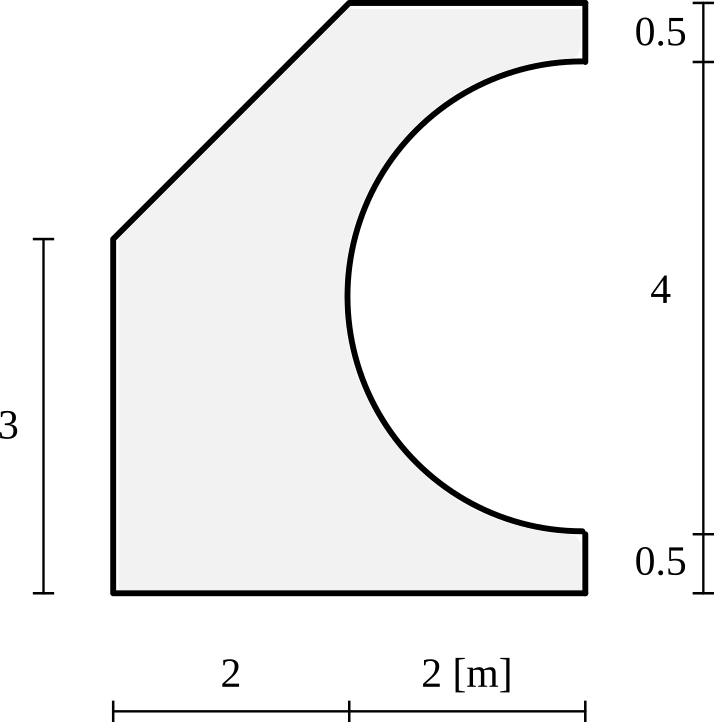
\includegraphics{SrodkiCiezkosci/Figura01.png}
    \caption{Blacha jednorodna z wycięciem}
\end{figure}

\begin{figure}[htbp]
    \centering
    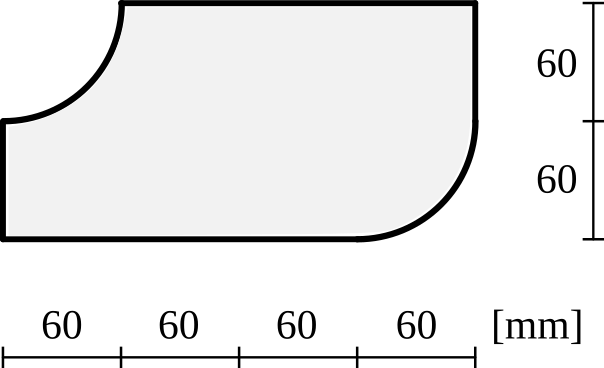
\includegraphics{SrodkiCiezkosci/Figura02.png}
    \caption{Blacha jednorodna z zaokrągleniami}
\end{figure}

\begin{figure}[htbp]
    \centering
    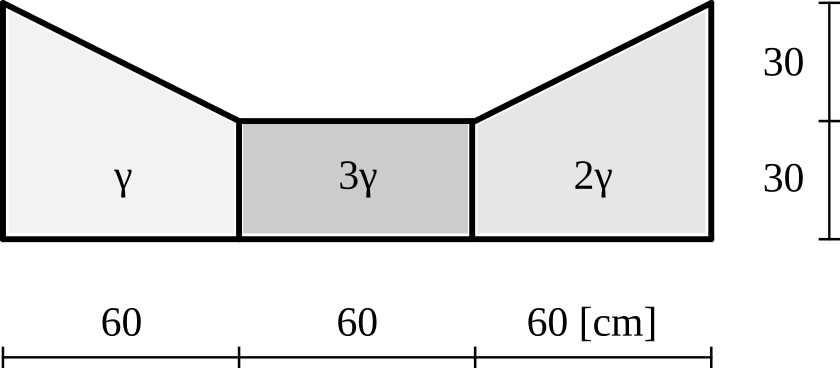
\includegraphics{SrodkiCiezkosci/Figura03.png}
    \caption{Blacha niejednorodna}
\end{figure}

\begin{figure}[htbp]
    \centering
    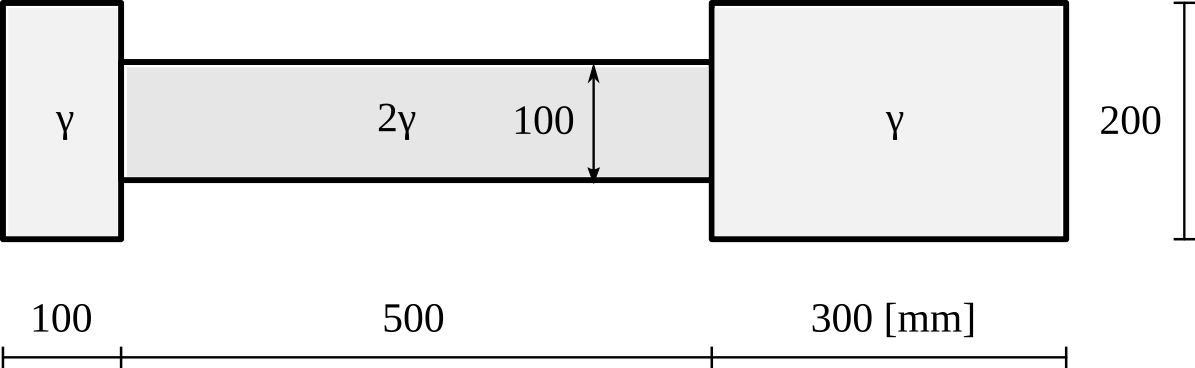
\includegraphics{SrodkiCiezkosci/Figura04.png}
    \caption{Blacha niejednorodna}
\end{figure}